% Grossmont College -- Chem 141: Periodicity of Chemical Properties
% Cameron Carroll
% May 2014


\documentclass[fleqn,titlepage]{article}

\renewcommand*\rmdefault{ppl}

\usepackage[version=3]{mhchem} % Package for chemical equation typesetting
\usepackage{tabu}
\usepackage{wasysym}
\usepackage{listings}
\usepackage{scrextend}
\lstset{language=Matlab}
\usepackage{multirow}
\usepackage{hyperref}

% set 1" margins on 8.5" x 11" paper
% top left is measured from 1", 1"
\topmargin 0in
\oddsidemargin 0in
\evensidemargin 0in
\headheight 0in
\headsep 0in
\topskip 0in
\textheight 9in
\textwidth 6.5in

\usepackage{graphicx} % Required for the inclusion of images

\setlength\parindent{0pt} % Removes all indentation from paragraphs

\renewcommand{\labelenumi}{\alph{enumi}.} % Make numbering in the enumerate environment by letter rather than number (e.g. section 6)

%\usepackage{times} % Uncomment to use the Times New Roman font

%----------------------------------------------------------------------------------------
% DOCUMENT INFORMATION
%----------------------------------------------------------------------------------------

\begin{document}

\begin{titlepage}
  \mbox{}\\[1.25cm]
  \textbf{\LARGE Cameron Carroll \\ Grossmont College}\\[2.25cm]
  \begin{center}
    \textbf{\huge Lab 9: \\ Periodicity of Chemical Properties}\\[2.50cm]
  \end{center}
  \textbf{\LARGE Professor: Martin Larter \\ Chemistry 141-0692} \\
  \vfill
  
  \center{\textbf{\LARGE Performed --} {\LARGE March, 2014}}
  \center{\textbf{\LARGE Submitted --} {\LARGE May 28, 2014}}
\end{titlepage}

%----------------------------------------------------------------------------------------
% SECTION 1
%----------------------------------------------------------------------------------------
\section*{}
  \begin{description}
    \item[Trend Examined:] Atomic Number versus Density
    \item[Description of Property:] The density of an element is its mass divided by its atomic volume, determined from atomic radius. It is essentially the amount of matter packed into a unit volume.
    \item[Summary:] \paragraph{} Generally speaking, density increases with atomic number, however there is a secondary trend where density rises and falls within a period. This shows that the mass term dominates over the `number density.' (1) \\
    The graph doesn't show a linear relationship, however... as I suspected and observed, increasing metallic character also increases density, apparently due to the metallic interactions. (1) -- Thanks to this, the general trend is increasing but with sub-peaks as you move across a period.
    \item[Graph:] (No more time to typset this and it wouldn't fit: graph follows.)
    \item[Discussion:] The general trend shows that mass increases more quickly than atomic radius. This follows from atomic shielding, where the number of protons is consistently increasing but the valence electrons are shielded somewhat from this by the core electrons. \\
    The amount of density increase from one atom to the next decreases as we move along a period, which is a result of more nonshielding valence electrons being added: More unshielded electrons means a higher atomic radius to go along with the extra proton. Upon reaching the end of a period, these valence electrons join the core -- The charge felt by valence electrons (and the number of valence electrons) show a clear drop on the graph. \\
    Finally, the secondary trend is a result of metallic character (1) where interactions between metallic atoms decrease the atomic radius (particularly transition metals, as the graph increases until peaking at the transitions, then decreasing to the noble gases.)
    \item[References:] 
      \begin{itemize}
        \item (1) \url{http://physics.stackexchange.com/questions/4234/why-is-the-relationship-between-atomic-number-and-density-not-linear}
      \end{itemize}
  \end{description}
  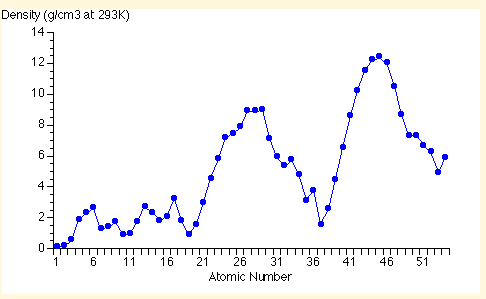
\includegraphics{./an_density}

\section*{Element Biography: Molybdenum}
  \paragraph{} Molybdenum, (Mo, 42) is a transition metal first isolated in 1781 by Peter Jacob Hjelm. It isn't found as a free metal, only in oxidated states inside of minerals. It's used particularly in creating steel alloys because of its ability to form carbides in iron alloys. \\
  Previously known as Molybdena, this element was confused with and used as graphite for blackening surfaces. Reportedly it was used in a steel alloy for a Japanese sword in the 14th century. Eventually it was discovered that it wasn't the same as graphite and was isolated using carbon and linseed oil. \\
  For an entire century after isolation, however, there was no industrial use for the element. Early alloys were hampered by their brittleness, despite the promise of hardening the alloy. Eventually, William Coolidge filed a patent for a process to make Molybdenum ductile in 1906. This allowed it to be used as a heating element in furnaces and a support in light bulbs. \\
  Use of the element spiked during World War I: It was used in steels for armor plating, replacing three times the thickness of less effective manganese steel alloy. Demand plummetted again until World War II, when it again saw strategic importance. \\
  The element is found primarily in MoS2, molybdenite, which is mined in Norway, Colorado and British Colombia, and is currently used primarily as an alloying material but also in chemical applications. It is even used as fertilizer in some cases, used in growing cauliflower.



\end{document}